% should we use RF or Random Forest ? ==> sometimes it looks/reads strange, not sure
% done, maybe mention that the position is a powerfull feature, but also a restriction/big assumptio
% done, mention the 0.95 DICE target
% done, autoref for subimages works different (no 'Figure')
% done, we only mention the rebustness in discussion but not the accuracy (that has not fullfiled)
% mention that we tried a little bit with SSM and 3D features ? ==> I wouldn't because it's not part of our solution
% mentioned that the samples are equally drawn from positive and negative samples

\documentclass[journal]{IEEEtran}

\usepackage[hidelinks]{hyperref}

\usepackage[pdftex]{graphicx}
\graphicspath{{figures/}}
\DeclareGraphicsExtensions{.pdf,.jpeg,.png}

\usepackage{subfig}

% Bibliography
\usepackage[backend=bibtex, style=ieee]{biblatex}
\addbibresource{sources.bib}

\title{Personalized Femoral Implant Planning by Automatic Distal Femur Segmentation}
\author{Iwan Paolucci, Severin Tobler\\The Tree Nurses}

\begin{document}

\markboth{Medical Image Analysis Lab, January~2016}

\maketitle

\begin{abstract}

\end{abstract}

% !TeX spellcheck = en-GB
\section{Introduction}
\IEEEPARstart{P}{ersonal} femoral implants feature less attrition, therefore more comfortable wearing and lower implant related issues after implantation. Furthermore the operation can be carried out more swiftly, if the implant is pre-operational adjusted to the patient. The personalisation of femoral implant requires an accurate segmentation of the femur. With an upcoming awareness of radiation, the trend of segmenting bones with MRI instead of CT data is increasing.
In this work we propose a fast and robust automatic femur segmentation from MRI data. The automatic segmentation is based on a Random Forest (RF) classifier and does not require any manual interaction. In the following sections the segmentation pipeline, the training and testing of the segmentation and the performance of the segmentation are described and discussed.

% Abstract:
% In this work we propose a fast and robust automatic femur segmentation from MRI data, in order to manufacture personal femoral implants.

% !TeX spellcheck = en-GB
\section{Materials \& Methods}
The automatic segmentation evolves around a Random Forest classifier. In \autoref{fig:pipeline} the whole segmentation pipeline is shown. The individual parts of the segmentation are covered in the following subsections. Furthermore the validation of the automatic segmentation is described.

To train the RF and evaluate the performance of the segmentation two data sets are used. The first data set comprises 20 MRI volumes and their ground truth. This data set is used to train the RF and evaluate quantitative the segmentation. The second data set contains 10 MRI volumes without ground truth, which are used to evaluate the segmentation qualitative.
\subsection{Pre processing}
In order to compensate for different MRI grey-scale representations, the images are normalized using z-score normalisation (\autoref{eq:zscorenormalize}). In a second step a Wiener filter is applied to reduce noise. This yields a normalized representation of the data, that is used for the next steps.
\begin{equation}
I_n = \frac{I - \mu}{\sigma}
\label{eq:zscorenormalize}
\end{equation}
\subsection{Feature Extraction \& Random Forest}
Thirteen different features are extracted for each voxel of the normalized data, which are used to apply the RF. The features cover different aspects of the data. To describe vertical and horizontal edges we use Prewitt and Sobel. The derivatives are covered by Laplacian and Laplacian of Gaussian and the intensity by Gaussian and Average filters. The statistical information is represented by the entropy and the standard deviation features. To restrict the classifier to the femur we added the relative position in 3D, with the strong assumption that the femur rotates and moves only slightly between the different MRI volumes. This assumption can be made, because the orientation of the patient in medical images is known according to the DICOM standard\cite{dicom-orientation}. To compensate for different image resolutions the relative position is used instead of the absolute.

The RF tree model is created by training a RF with 15 trees on 1\% of the voxels from the training images, which are randomly picked. Applying the RF tree model on the extracted features yields the segmented femur.
%We used 13 different features of which we had edge representations like Prewitt and Sobel, derivatives using the Laplacian and Laplacian of Gaussian and intensity information using Gaussian and Average filters. Additionally we added statistical information entropy and standard deviation. To restrict the classifier to the Femur, we added the relative position in 3D. The relative position is used instead of the absolute, to compensate for different image resolutions.
%The RF classifier is trained using 15 trees and 1\% of the voxels from the training images, which are randomly picked. 
\subsection{Post processing}
After the prediction of the Random Forest classifier, the results are post processed to remove outliers. The implemented post processing comprises following four steps, where the 2D operations are applied on each slice and the 3D operation on the volume:
\begin{enumerate}
\item 2D Morphological opening
\item 2D Keep largest area
\item 2D Morphological filling
\item 3D Keep largest volume
\end{enumerate}
Applying this four steps yields the final segmented volume. In order to present the result, the volume is converted to a mesh by applying a marching cubes algorithm \cite{lorensen}. 
\subsection{Validation}
To validate the whole segmentation, a randomized 5-fold cross validation \cite{cross} is used on the first data set. Out of the 20 volumes 16 are used to train and 4 to test the algorithm. To measure the accuracy and robustness the mean DICE coefficient\cite{powers2011evaluation} and the standard deviation over all 20 results is used.
\begin{figure*}[!t]
\centering
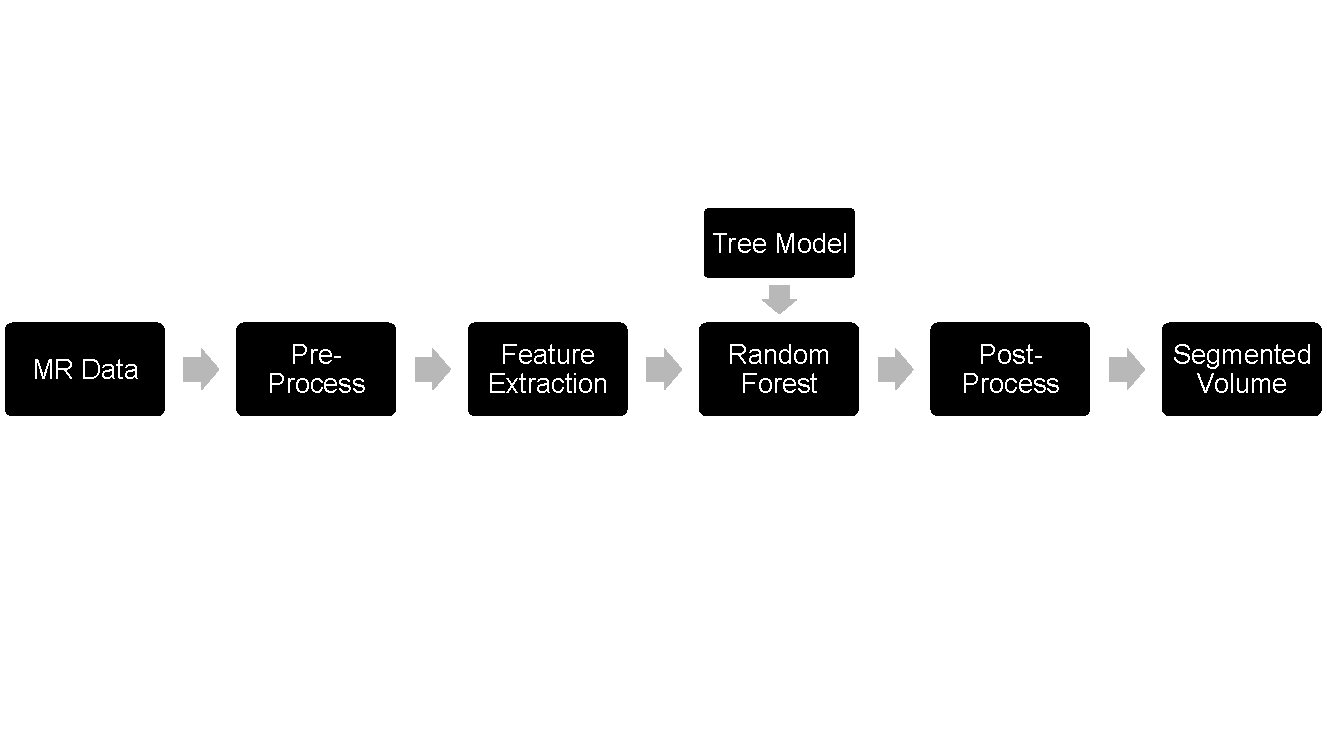
\includegraphics[width=\textwidth]{pipeline}
\caption{Pipeline of the automatic segmentation using a Random Forest model to segment the femur from MRI data, followed by postprocessing and visualization using marching cubes.}
\label{fig:pipeline}
\end{figure*}

%fully automatic
%show the pipeline
%preprocessing (normlization, wiener filer), maybe show picture
%training, features, relative position, show kernels, number of trees, 2d features
%postprocessing, opening, largest area, filling, largest volume, show images as in presentation
%explain our cross validation procedure (DICE not OOB score)


% !TeX spellcheck = en-GB
\section{Results}
The 5 fold cross validation of the proposed algorithm, resulted in a mean DICE of $0.91$ with a standard deviation of $0.03$. This can be graphically seen in \autoref{fig:dicecrossvalid}. The range lies between $0.85$ and $0.96$ and has a median of $0.9$. The average computation time for the whole algorithm is $2.5$ minutes.
\begin{figure}[h]
\centering
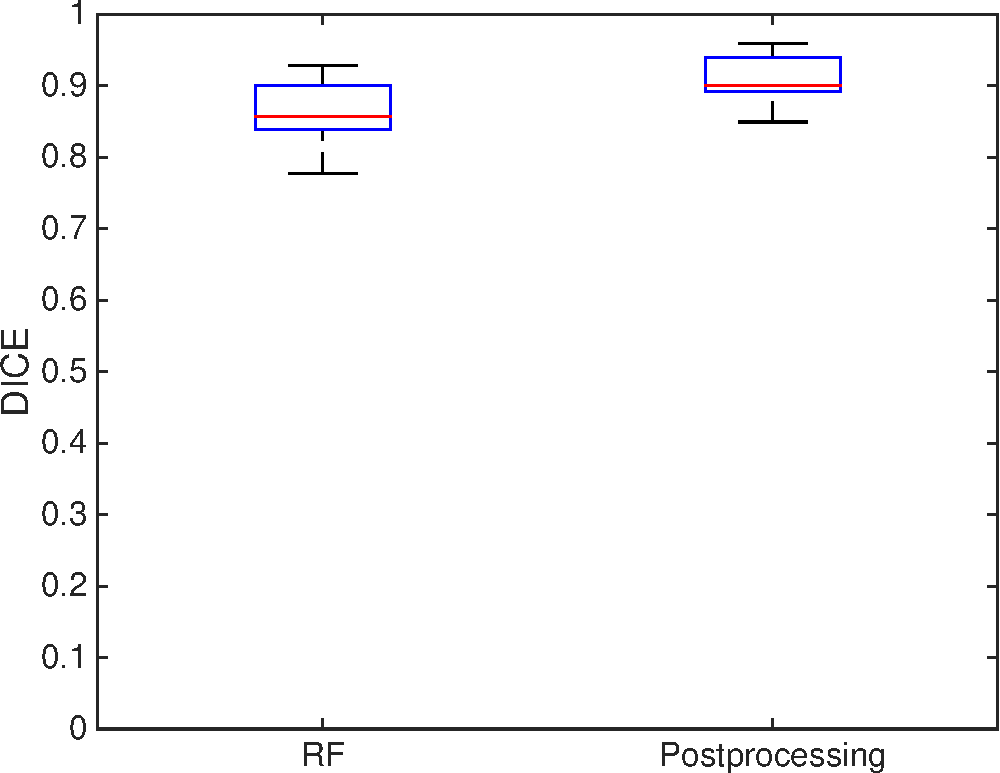
\includegraphics[width=0.9\linewidth]{dicecrossvalid.pdf}
\caption{DICE}
\label{fig:dicecrossvalid}
\end{figure}

In \autoref{fig:bestcase} and \autoref{fig:worstcase} the optically best and worst result out of the test data are shown.
\begin{figure*}[!t]
	\centering
	\subfloat[Bestcase result of the test data (Image 29)]{
		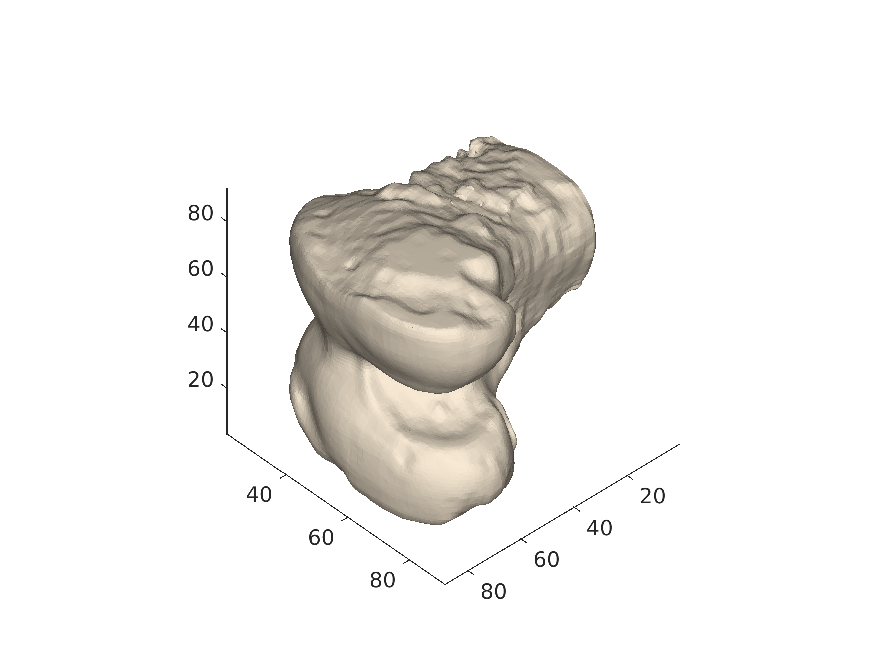
\includegraphics[width=0.48\textwidth]{vr029}
		\label{fig:bestcase}}
	\hfil
	\subfloat[Worstcase result of the test data (Image 21)]{
		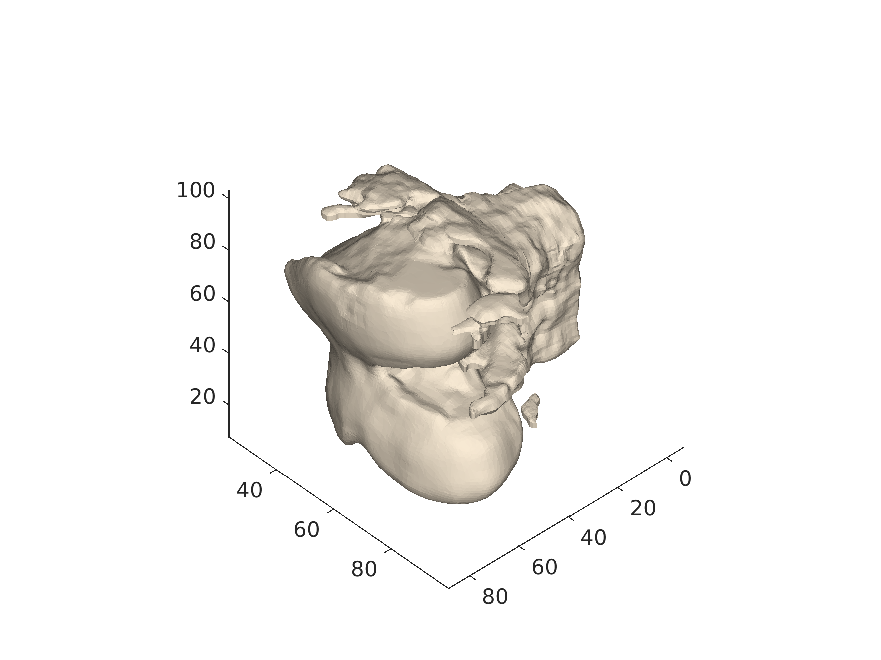
\includegraphics[width=0.48\textwidth]{vr021}
		\label{fig:worstcase}}
\end{figure*}

% !TeX spellcheck = en-GB
\section{Discussion}
The results in \autoref{fig:dicecrossvalid} with a standard deviation of 0.03 let us conclude, that we achieved our goal of a robust algorithm, which we set with 0.05 standard deviation. We validated our algorithm with a 5 fold cross validation, to ensure the algorithm is tested on MRI volumes, that have not been used for training. Therefore we can expect it to perform with the same accuracy on new data and not to have overfitting of our Random Forest model. With an accuracy of 0.91 DICE the goal of a of 0.95 has not been reached. 

In order to use the algorithm for femoral implant planning, mainly the condyles have to be segmented well. With the 3D volume rendering from the best case result in \autoref{fig:bestcase} it is possible to measure distances between important structures to plan a femoral implant. However, the epicondyles are not fully segmented, which is something that has to be improved in the future. In the case of \autoref{fig:worstcase} one could do the required measurements, although there are lots false positives. However, the accuracy is probably not high enough for clinical routine.

In \autoref{fig:worstcase} the worst case result is shown. This particular case could have yielded better results with a more aggressive post processing approach. By applying the morphological opening with a bigger kernel the false positives could have been reduced. Because a bigger kernel would be able to split the connection from the bone to the artefacts. The separated artefacts are then discarded by keeping only the largest volume in the next post processing step. Nonetheless, this approach would also remove true positives and over all lower the segmentation performance in other images. 

As mentioned in the beginning, our main goal is to develop a robust algorithm. This has been achieved by keeping the algorithm simple, which prevents overfitting and long segmentation time. Therefore all steps that worsened the results in some cases have been removed. As an example we did not include skewness as a feature, as it worsened the results slightly in more than half of the cases.

% !TeX spellcheck = en-GB
\section{Conclusion}
We developed a fast and robust automatic segmentation. The loading of one MRI volume until the final segmentation requires in average $2.5$ minutes on a commercial laptop. With a DICE of $0.91$ and a standard deviation of $0.03$ the segmentation has a sufficient robustness, but lacks in accuracy.

In order to enhance the accuracy, we propose to include prior information of the patent. One could create several Random Forest models for specific group of people, where the groups differ in age, sex, weight or height. Prior information could also be considered by supporting the segmentation with a Statistic Shape Model \cite{heimann2009statistical}. However the performance of the Statistic Shape Model depends strongly on its initialization and may therefore decrease the robustness of the segmentation.
An other potential way to increase the accuracy is to exchange the 2D features of the Random Forest by 3D features. This might represent the data better, since an additional dimension is considered. The challenge is that the slice spacing is multiple times bigger than the pixel spacing. The feature kernels must therefore be adjusted and this might end up loosing properties like separability.


\printbibliography

\end{document}


